\documentclass[preprint,12pt]{elsarticle}

%% Use the option review to obtain double line spacing
%% \documentclass[preprint,review,12pt]{elsarticle}

%% Use the options 1p,twocolumn; 3p; 3p,twocolumn; 5p; or 5p,twocolumn
%% for a journal layout:
%% \documentclass[final,1p,times]{elsarticle}
%% \documentclass[final,1p,times,twocolumn]{elsarticle}
%% \documentclass[final,3p,times]{elsarticle}
%% \documentclass[final,3p,times,twocolumn]{elsarticle}
%% \documentclass[final,5p,times]{elsarticle}
%% \documentclass[final,5p,times,twocolumn]{elsarticle}

%% The graphicx package provides the includegraphics command.
\usepackage{graphicx}
%% The amssymb package provides various useful mathematical symbols
\usepackage{amssymb}
\usepackage{amsmath}
\usepackage{breqn}
\usepackage{chemfig}
\usepackage{csvsimple}
%% The amsthm package provides extended theorem environments
%% \usepackage{amsthm}

%% The lineno packages adds line numbers. Start line numbering with
%% \begin{linenumbers}, end it with \end{linenumbers}. Or switch it on
%% for the whole article with \linenumbers after \end{frontmatter}.
\usepackage{lineno}
\usepackage{natbib}
\usepackage{hyperref}
% \usepackage[top=0.75in, bottom=0.75in, left=0.55in, right=0.85in]{geometry}
\usepackage{graphicx}
\usepackage{url}
\usepackage{palatino}
\usepackage{tabularx}
\usepackage{graphicx}
\usepackage{multicol}
\usepackage{graphicx}
\usepackage{amssymb}
\usepackage{float}
\usepackage{amsmath}
\usepackage{rotating}
\usepackage{subfigure}
\usepackage{multirow}
\usepackage{mathrsfs}
\usepackage{xfrac}
\usepackage[font=small,skip=0pt]{caption}
%\usepackage[numbers,sort&compress]{natbib}
%\usepackage{hyperref}
\usepackage{pgf,tikz}
\usetikzlibrary{shapes,arrows,chains}
\usetikzlibrary[calc]
\usepackage{graphicx}
\graphicspath{ {./plotting_files/} }

\usepackage{geometry}
\geometry{lmargin=1in,rmargin=1in,tmargin=1in,bmargin=1in}
\usepackage{lipsum}
%\pagestyle{empty}
\usepackage{natbib}
\pagenumbering{arabic}
%\usepackage[T1]{fontenc}
\usepackage{setspace}
\usepackage{mathptmx}
\usepackage{t1enc}
%\usepackage{xkeyval}
%\usepackage{chemformula}
%\usepackage{array}
%\usepackage{booktabs}
%\usepackage{hypdoc}
%\usepackage{listings}
%\usepackage{lmodern}
%\usepackage{mathpazo}
%\usepackage{microtype}
\usepackage{graphicx}
\usepackage{amssymb}
\usepackage{float}
\usepackage{amsmath}
\usepackage{rotating}
\usepackage{subfigure}
\usepackage{multirow}
\usepackage{xfrac}
\usepackage[font=small,skip=0pt]{caption}
%\usepackage[numbers,sort&compress]{natbib}
%\usepackage{hyperref}
\usepackage{pgf,tikz}
\usetikzlibrary{shapes,arrows,chains}
\usetikzlibrary[calc]
\usepackage{graphicx}
\usepackage{geometry}
\geometry{lmargin=1in,rmargin=1in,tmargin=1in,bmargin=1in}
\usepackage{lipsum}
%\pagestyle{empty}
\usepackage{natbib}
\pagenumbering{arabic}
%\usepackage[T1]{fontenc}
\usepackage{setspace}
\usepackage{mathptmx}
\usepackage{t1enc}
%\usepackage{xkeyval}
%\usepackage{chemformula}
%\usepackage{array}
%\usepackage{booktabs}
%\usepackage{hypdoc}
%\usepackage{listings}
%\usepackage{lmodern}
%\usepackage{mathpazo}
%\usepackage{microtype}
\usepackage{lineno,hyperref}
\usepackage{multirow}
\usepackage{cancel}
\usepackage{url}
\usepackage[norule]{footmisc}
\usepackage[utf8]{inputenc}
\usepackage[english]{babel}
\hypersetup{colorlinks = true,linkcolor = blue,urlcolor = blue}
% \fontfamily{SansSerif}
% \selectfont
% \usepackage[T1]{fontenc}
% \usepackage
%% natbib.sty is loaded by default. However, natbib options can be
%% provided with \biboptions{...} command. Following options are
%% valid:
%%   round  -  round parentheses are used (default)
%%   square -  square brackets are used   [option]
%%   curly  -  curly braces are used      {option}
%%   angle  -  angle brackets are used    <option>
%%   semicolon  -  multiple citations separated by semi-colon
%%   colon  - same as semicolon, an earlier confusion
%%   comma  -  separated by comma
%%   numbers-  selects numerical citations
%%   super  -  numerical citations as superscripts
%%   sort   -  sorts multiple citations according to order in ref. list
%%   sort&compress   -  like sort, but also compresses numerical citations
%%   compress - compresses without sorting
%%
%% \biboptions{comma,round}
% \biboptions{}

\usepackage{caption}
\usepackage{algorithm} 
\usepackage[noend]{algpseudocode}
\usepackage{amsmath}
\DeclareMathOperator*{\argmin}{argmin}
\DeclareMathOperator*{\argmax}{argmax}
\newcommand*{\argminl}{\argmin\limits}
\newcommand*{\argmaxl}{\argmax\limits}



\begin{document}
	
	\begin{frontmatter}
		
		%% Title, authors and addresses
		
		\title{CS6700 : Reinforcement Learning
			\\Programming Assignment : 1}	
		\author{Pragneshkumar Rana - ME17301}

		\address{Indian Institute of Technology, Madras}

		\begin{abstract}
			%% Text of abstract
		 Experiment of 10 arm-bandit testbed was conducted to find out optimal strategy. Greedy approach, soft-max exploration, Upper confidence bound and Median elimination algorithm are discussed here. The objective of this algorithm to identify the maximum reward given set of trials by trade-off between exploration and exploitation.  
		\end{abstract}
		
		\begin{keyword}
			Greedy approach, Soft-max exploration, Upper confidence bound, Median elimination algorithm , Multi-arm bandit
			%% keywords here, in the form: keyword \sep keyword
			
			%% MSC codes here, in the form: \MSC code \sep code
			%% or \MSC[2008] code \sep code (2000 is the default)
		\end{keyword}
		
	\end{frontmatter}
	
	%%
	%% Start line numbering here if you want
	%%

	
	%% main text
	\section{(Q:1) $\epsilon$ - greedy:}
	\label{S:1}
	Ref: \cite{sutton2018reinforcement} 
	\cite{vidya}
	
	$\epsilon$- greedy algorithm was implemented on 10-arm testbed. The simulation run for 1000 different steps in which each step gives reward based on the randomly picked arm and its associated probability distribution $\mathcal{N}$(Distribution associated with arm,1). Same procedure was repeated for 2000 different bandit problems in which each of the 10-arm has distribution from $\mathcal{N}$(0,1). 
	
	The expected performance of $\epsilon$-greedy algorithm was obtained on different $\epsilon$ value. In which $\epsilon$ times exploration happens and $1-\epsilon$ times exploitation was done. Experiments was conducted with values of $\epsilon=[0,0.02,0.1,1]$. As mention earlier generated graphs are average over 2000 different bandit runs.
	
	The figure-$\ref{fig1:greedy_rew}$ first graph shows that with $\epsilon = 0$, for fully greedy simulation ended up in sub-optimal exploitation with average reward  1 whereas it clear from the graph that maximum reward can be obtained around 1.5. With slight increase in $\epsilon=0.02$ increment in reward is quite high. Further increment in $\epsilon=0.1$ did not give much increment, which shows the trade off between the exploration and exploitation.
	$epsilon=1$ shows if you do extreme level of exploration then the average reward fluctuates lot and expected reward is least.
	
	The similar observation can be obtain from the figure-$\ref{fig2:greedy_opt}$. Second graph shows that with $\epsilon =0$ the optimal arm is chosen $\approx \frac{1}{3}$ times whereas non-optimal arms are picked up around $\approx \frac{2}{3}$ times. With $\epsilon=0.02$, given chance of exploration, chance of picking the optimal arm also increases. With $\epsilon=0.1$  chance of picking the best arm is around 80$\%$. But $\epsilon=1$ it explores all the arm equally likely so, given 10 arm the optimal arm is picked up around 10$\%$ of the times.
	
	
	 \begin{figure}[H]
	 	\centering
	 	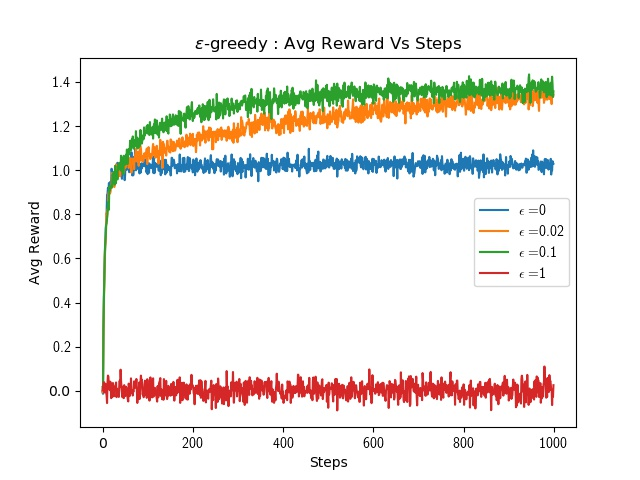
\includegraphics[scale=0.7]{./reward_epsilon.jpg}
	 	\hspace{0.25cm}
	 	\caption{Average performance on REWARD using $\epsilon$ greedy algorithm over 2000 different 10-armed bandit problem}
		 \label{fig1:greedy_rew}
	 \end{figure}
	 
	 
	 \begin{figure}[H]
	 	\centering
	 	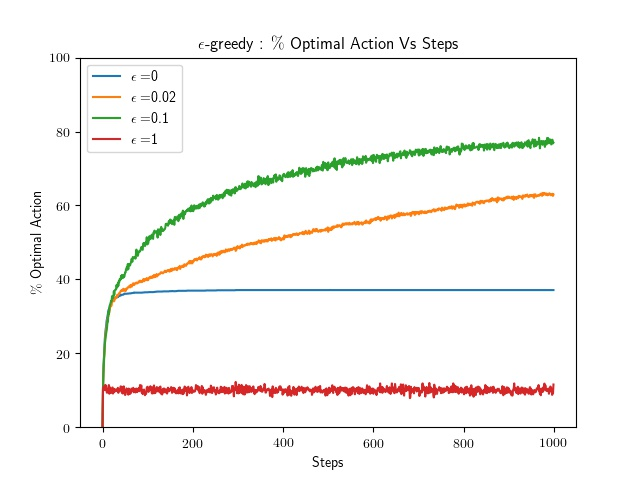
\includegraphics[scale=0.7]{./optimal_epsilon.jpg}
	 	\hspace{0.25cm}
	 	\caption{Average performance on OPTIMAL ACTION using $\epsilon$ greedy algorithm over 2000 different 10-armed bandit problem}
	 	\label{fig2:greedy_opt}
	 \end{figure}
	 
	 \newpage
	 
 	\section{(Q:2)  Softmax Algorithm:}
 	\label{S:2}
 	
 	Softmax algorithm was implemented on Gibbs distribution on similar problem of 10 arm test-bed. Simulator run for 1000 steps and 2000 different bandit problem. 
 	
 	The empirical formula of softmax is used to find out the probability based on the reward.
 	
 	\begin{equation}
 		p_{i} (t+1)=  \frac{\exp({\frac{Q(t)}{\tau}})}{\sum_{i} \frac{Q_i(t)}{\tau} }
 	\end{equation}
 	
 	 From obtained probability using soft-max, random values was picked up from the distribution and associated arm-index was obtained from it.\textbf{ In epsilon-greedy algorithm, in exploration stage all the arms has equal probability to get selected which is quite unfair as bad arm has same probability as best arm. To overcome this problem gibbs distribution is used to probability generated based on past rewards which gives more weightage to the arm with better rewards. so, Gibbs distribution is fair on the 10-arm testbed.}
 	 
 	 
	Temperature parameter  in softmax algorithm controls the randomness of the choice. Simulation has been done using temperature-$\tau =[0.02,0.1,0.5,10]$.  When $\tau \rightarrow 0$ softmax act as almost greedy algorithm. Whichever arm has highest reward will get highest probability. 
 	 
 	 
 	 From the figure-$\ref{fig1:soft_raw}$ it can be observed that, for $\tau=0.02$ the average reward obtain is around 1 which same as pure greedy algorithm reward. For $\tau=0.1$ Average reward is maximum around 1.4 but as $\tau$ increases expected reward decreases and for very high value of $\tau=10$ more exploration took place so average reward is least in that case.
 	 
 	 From figure-\ref{fig2:soft_opt}, it clear that for very low value $\tau$, optimal arm was picked up around $\frac{1}{3}$ times. For slightly high value of $\tau = 0.1 and 0.5$ optimal arm was picked up aound 60\% times. But very high value of temperature causes more exploration and due to high exploration all arm were equally picked up so, optimal arm was picked up around 10\% times.
 	 
 	 \begin{figure}[H]
 	 	\centering
 	 	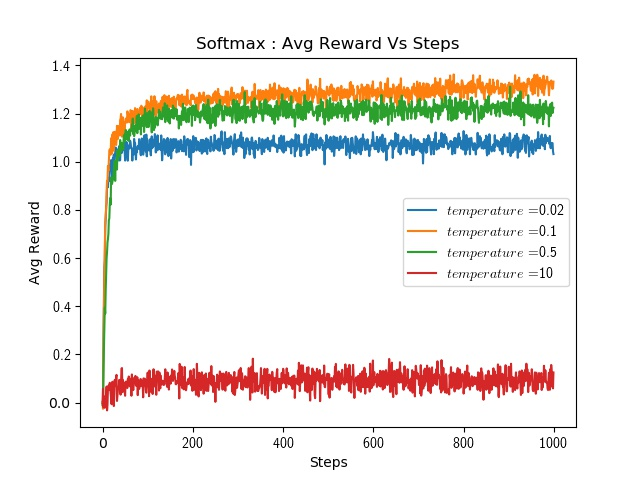
\includegraphics[scale=0.7]{./reward_soft.jpg}
 	 	\hspace{0.25cm}
 	 	\caption{Average performance on REWARD using softmax algorithm over 2000 different 10-armed bandit problem}
 	 	\label{fig1:soft_raw}
 	 \end{figure}
 	 
 	 
 	 \begin{figure}[H]
 	 	\centering
 	 	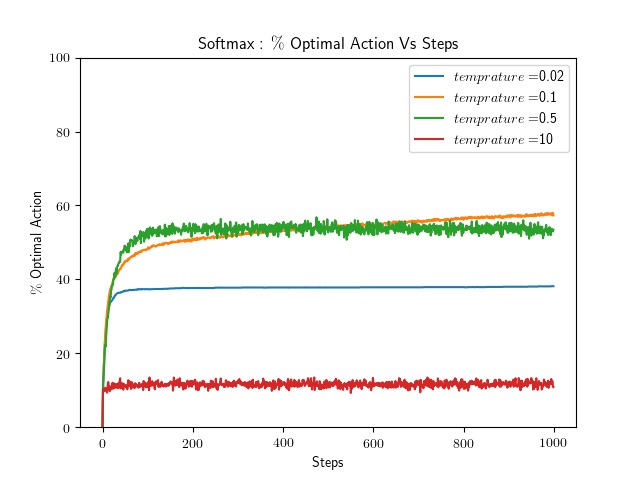
\includegraphics[scale=0.7]{./optimal_soft.jpg}
 	 	\hspace{0.25cm}
 	 	\caption{Average performance on OPTIMAL ACTION using softmax algorithm over 2000 different 10-armed bandit problem}
 	 	\label{fig2:soft_opt}
 	 \end{figure}
 	 
 	 
 	 \section{(Q:3)  UCB-1 Algorithm:}
 	 \label{S:3}
 	 
 	 UCB-1 algorithm was implemented on 10-armed testbed, for which it run for 1000 steps and expected performance over 2000 bandit problem was compared with $\epsilon- greedy$ and Softmax algorithm. UCB1 algorithm is a famous as used the fact that any system output has always uncertainty associated with the expected value of reward which generates need of exploration.The concept is to select non optimal
 	 arms according to their potential for actually being optimal, by considering closeness of their maximal mean estimates and uncertainties.
 	 
 	 \begin{equation}
 	 	A_t = \argmax \bigg [Q(t) + c *\sqrt{\frac{\ln{t}}{N_t(a)}} \bigg]
 	 \end{equation}
 	 
 	 where, 
 	 
 	 $N_t(a)$ denotes the number of times that action a has been selected prior to time t, 
 	 
 	 $Q_t(a)$ is the mean estimate of arm a, 
 	 the number c > 0 controls the degree of exploration.
 	 
 	 In this equation square root term, determines the uncertainty associated in the estimation of a.Lower value $N_t(a)$ in denominator shows the higher uncertainty means the arm which pulled less time has poor estimate of mean with high uncertainty. so we should pull the arm a which increases $N_t(a)$ and reduces uncertainty. This guarantees that all arms will eventually be pulled, and arms with lower value
 	 estimates will be selected less frequently and optimal arm should be pulled more frequently.
 	 
 	 from the figure-\ref{fig1:ucb_raw} we can observe that UCB1 performs better than $\epsilon -greedy$ \& softmax algorithm except in the initial stage due to high variance with optimal reward it select arm randomly. \\
 	 
 	 For almost all parameter this algorithm guarantee convergence unlike other algorithm in which proper parameter control is required.  
 	 
 	 From figure-\ref{fig1:greedy_rew},\ref{fig1:soft_raw},\ref{fig1:ucb_raw} it clear that for any moderate value of parameter algorithm performs better than $\epsilon -greedy$ \& softmax algorithm. For the worst case of parameter value 10 other algorithm did not give good expected reward but UCB give better than other even in worst case. UCB1 adjusts its upper confidence bound of each arm, which helps algorithm to do both exploration and exploitation for each arms, which makes UCB1 performance better than $\epsilon$ greedy \& softmax algorithm.
 	
	 \begin{figure}[H]
		 	\centering
		 	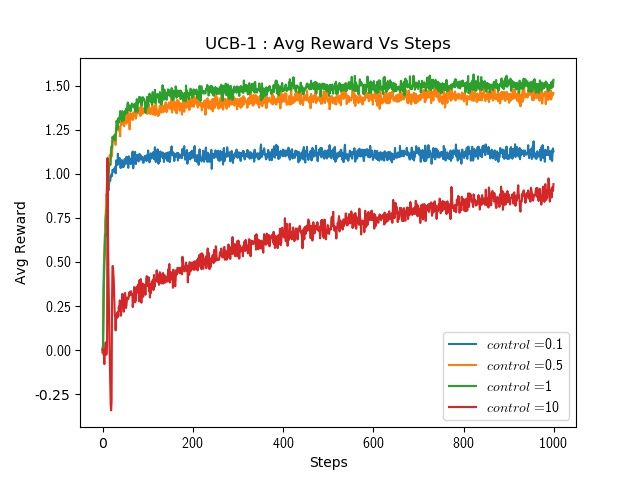
\includegraphics[scale=0.7]{./reward_ucb.jpg}
		 	\hspace{0.25cm}
		 	\caption{Average performance on REWARD using UCB-1 algorithm over 2000 different 10-armed bandit problem}
		 	\label{fig1:ucb_raw}
	 \end{figure}
	 
	 
	 \begin{figure}[H]
		 	\centering
		 	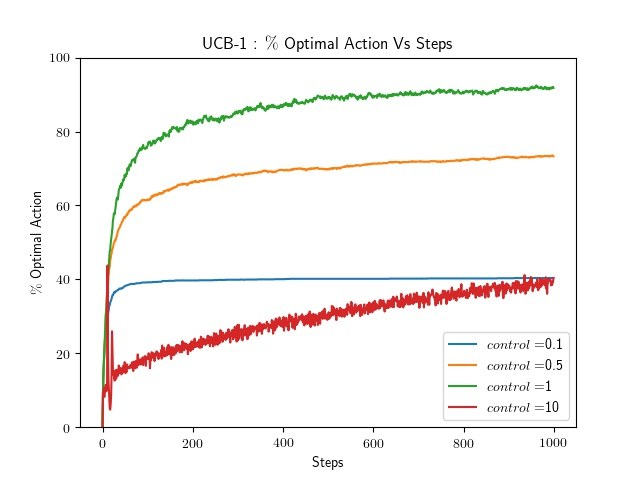
\includegraphics[scale=0.7]{./optimal_ucb.jpg}
		 	\hspace{0.25cm}
		 	\caption{Average performance on OPTIMAL ACTION using UCB-1 algorithm over 2000 different 10-armed bandit problem}
		 	\label{fig2:ucb_opt}
	 \end{figure}
	 
	 \section{(Q:5) For 1000 Arms:}
 	 \label{S:4}
 	 
	The result obtain by running the same simulation for 1000 arms are given in figures. By increasing the number of arms for same setup the obtained reward is quite high compared to other less number of arms but chances of selection of optimal arm in all cases is very less.
	
	 \begin{figure}[H]
	 	\centering
	 	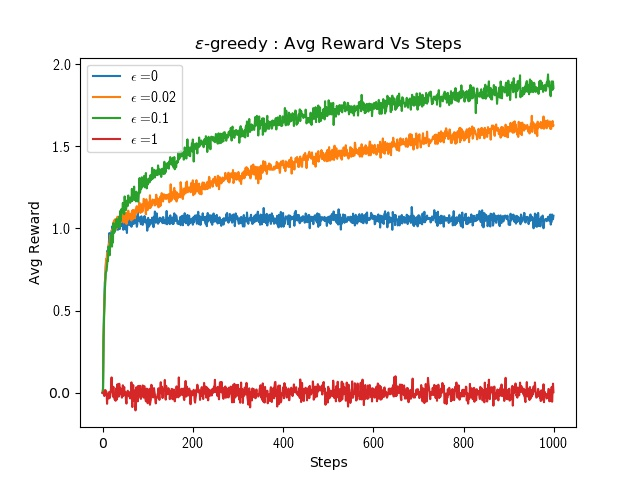
\includegraphics[scale=0.7]{./reward_epsilon_1000.jpg}
	 	\hspace{0.25cm}
	 	\caption{Average performance on REWARD using $\epsilon$ greedy algorithm over 2000 different 1000-armed bandit problem}
	 	\label{fig1:greedy_rew_1000}
	 \end{figure}
	 
	 
	 \begin{figure}[H]
	 	\centering
	 	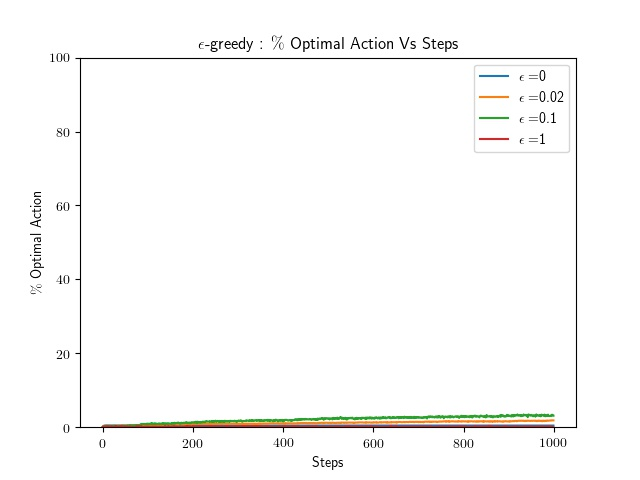
\includegraphics[scale=0.7]{./optimal_epsilon_1000.jpg}
	 	\hspace{0.25cm}
	 	\caption{Average performance on OPTIMAL ACTION using $\epsilon$ greedy algorithm over 2000 different 1000-armed bandit problem}
	 	\label{fig2:greedy_opt_1000}
	 \end{figure}
	
	 \begin{figure}[H]
		 	\centering
		 	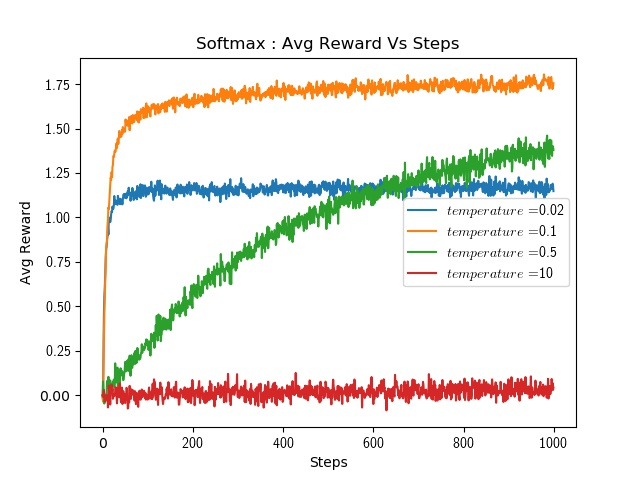
\includegraphics[scale=0.7]{./reward_soft_1000.jpg}
		 	\hspace{0.25cm}
		 	\caption{Average performance on REWARD using softmax algorithm over 2000 different 1000-armed bandit problem}
		 	\label{fig1:soft_raw_1000}
	 \end{figure}
	 
	 
	 \begin{figure}[H]
		 	\centering
		 	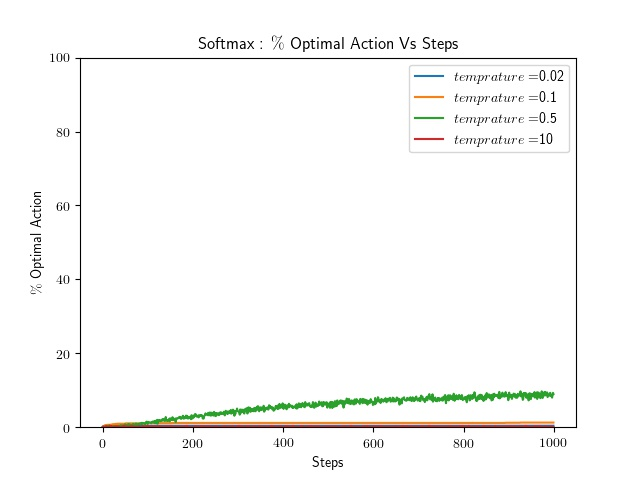
\includegraphics[scale=0.7]{./optimal_soft_1000.jpg}
		 	\hspace{0.25cm}
		 	\caption{Average performance on OPTIMAL ACTION using softmax algorithm over 2000 different 1000-armed bandit problem}
		 	\label{fig2:soft_opt_1000}
	 \end{figure}
		 
	
	\begin{figure}[H]
		\centering
		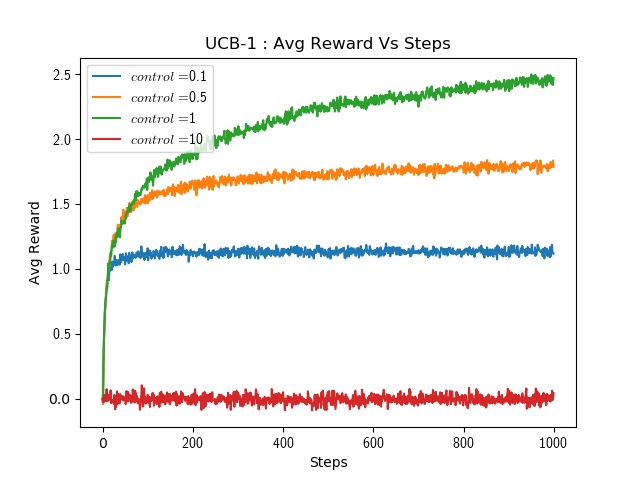
\includegraphics[scale=0.7]{./reward_ucb_1000.jpg}
		\hspace{0.25cm}
		\caption{Average performance on REWARD using UCB-1 algorithm over 2000 different 1000-armed bandit problem}
		\label{fig1:ucb_raw_1000}
	\end{figure}
	
	
	\begin{figure}[H]
		\centering
		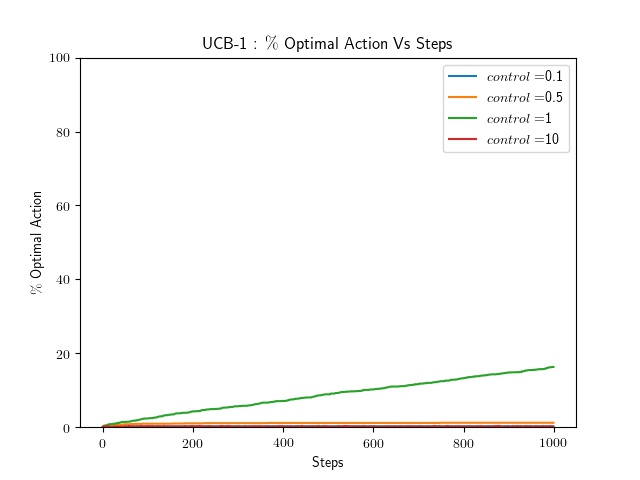
\includegraphics[scale=0.7]{./optimal_ucb_1000.jpg}
		\hspace{0.25cm}
		\caption{Average performance on OPTIMAL ACTION using UCB-1 algorithm over 2000 different 1000-armed bandit problem}
		\label{fig2:ucb_opt_1000}
	\end{figure}
	
	It clear from the graph that obtain reward in each case in high compared with its previous setup of less arms. For 1000 arms same result interpretation is obtained as before explained. In case average reward UCB gives maximum rewards. 
	
	For almost all parameter selection of optimal arm in $\epsilon - greedy $ algorithms is least compared to all algorithms. There is slight high chance of picking up optimal arm in soft-max algorithm for $\tau=0.5$ which at max pick optimal arm 10$\%$ in whole setup. UCB outperformance compared to all other algorithm. With number of increment in number of steps selection of optimal arm increases which clearly \textbf{shows that for more number of arms number of run/play required for all algorithm is quite high and UCB still performs better in all three algorithms.
}
				 
			\vspace{1cm}	
			References:
					%%
					%% Following citation commands can be used in the body text:
					%% Usage of \cite is as follows:
					
					%%   \cite{key}          ==>>  [#]
					%%   \cite[chap. 2]{key} ==>>  [#, chap. 2]
					%%   \citet{key}         ==>>  Author [#]
					
					%% References with bibTeX database:
					\bibliographystyle{ieeetr}
					\bibliography{biblio.bib}					
					%% Authors are advised to submit their bibtex database files. They are
					%% requested to list a bibtex style file in the manuscript if they do
					%% not want to use model1-num-names.bst.
					
					%% References without bibTeX database:
					
					% \begin{thebibliography}{00}
					
					%% \bibitem must have the following form:
					%%   \bibitem{key}...
					%%
					
					% \bibitem{}
					
					% \end{thebibliography}
					
					
				\end{document}
				
				%%
				%% End of file `elsarticle-template-1-num.tex'.